\subsection{Validazione}
\subsubsection{Scopo}
Questo processo assicura che il prodotto rispetti i requisiti e soddisfi le aspettative del proponente.

\subsubsection{Descrizione}
Per svolgere quanto sopra descritto usa come input l'output del processo di verifica,
restituendolo con la garanzia che soddisfi i requisiti.\\
Il principale attore è il \textit{Responsabile di Progetto}, il quale ha l'onere di decidere
se accettare e quindi approvare il prodotto oppure rigettarlo, indicando quali verifiche sono mancanti.

\subsubsection{Aspettative}
Per avviare il processo di validazione devono essere presenti questi elementi:
\begin{itemize}
    \item identificazione degli elementi da validare (documenti e/o codice sorgente)
    \item adottare una strategia di validazione che permetta di riutilizzare le procedure usate
    per la validazione
    \item valutazione dei risultati rispetto alle attese
\end{itemize}

\subsubsection{Validazione dei documenti}
\begin{figure}[h!]
    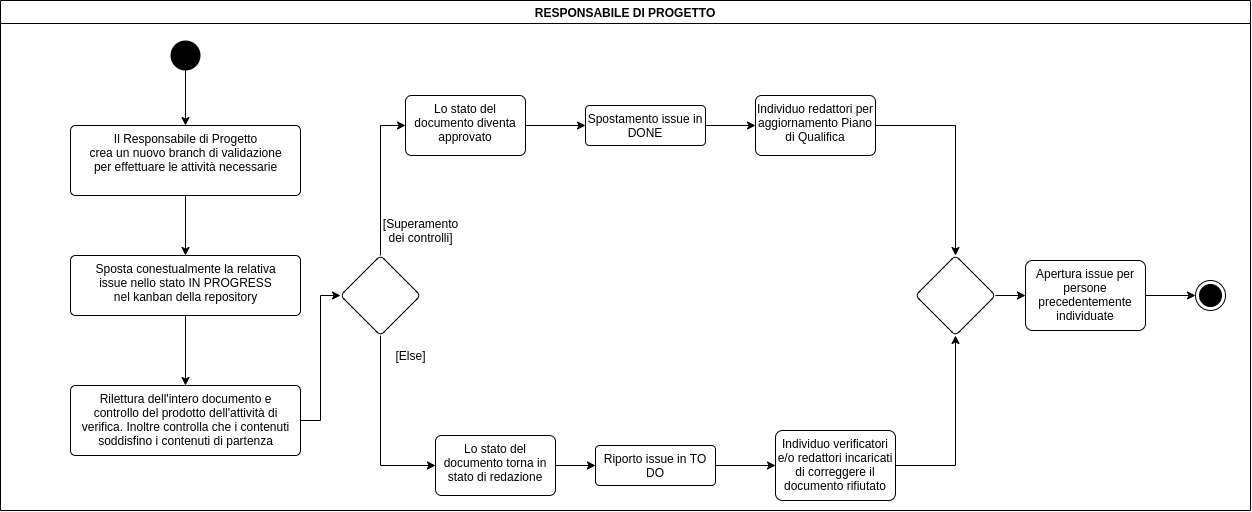
\includegraphics[width=\linewidth]{res/images/processo_validazione.png}
    \caption{Processo di validazione documenti}
\end{figure}
